\documentclass[a4paper,12pt]{article} % тип документа

% report, book

% Рисунки
\usepackage{graphicx}
\usepackage{wrapfig}
\usepackage{mathtext}

\usepackage{hyperref}
\usepackage[rgb]{xcolor}
\hypersetup{				% Гиперссылки
    colorlinks=true,       	% false: ссылки в рамках
	urlcolor=blue          % на URL
}

%  Русский язык

\usepackage[T2A]{fontenc}			% кодировка
\usepackage[utf8]{inputenc}			% кодировка исходного текста
\usepackage[english,russian]{babel}	% локализация и переносы


% Математика
\usepackage{amsmath,amsfonts,amssymb,amsthm,mathtools} 


\usepackage{wasysym}

\author{Анна Назарчук Б02-109}
\title{2.3.1a Современные средства получения и измерения вакуума}
\date{}
\begin{document}
\maketitle
\section{Аннотация}
Изучаются принципы получения и измерения вакуума
в экспериментальном стенде на основе компактного безмасляного высоковакуумного откачного поста, вакууметров.
Оборудование: турбомолекулярный насос HiPace 80, форвакуумный насос MVP 015, комбинированный вакуумметр MPT 100 (В2) типов Пирани (терморезисторный) и холодный катод (инвертированный магнетрон)ю

\section{Теоретические сведения}
\begin{equation}
S=\frac{dV}{dt}
\end{equation}
S - быстрота откачивающего действия вакуумной системы
Быстродействие насоса:
\begin{equation}
S_H = \frac{dV_H}{dt}
\end{equation}
Эффективная скорость откачки камеры:
\begin{equation}
S_0 = \frac{dV_0}{dt}
\end{equation}
Пропускная способность (проводимость):
\begin{equation}
U = \frac{Q}{P_1-P_2}
\end{equation}
Q - поток газа через вакуумпровод
Основное уравнение вакуумной техники:
\begin{equation}
\frac{1}{S_0} = \frac{1}{S_H}+\frac{1}{U} 
\end{equation}
Натекание - количественная характеристика течи:
\begin{equation}
Q_H = V\frac{P_K-P_H}{\Delta t}
\end{equation}
Число Кнудсена - степень разреженности газового
потока:
\begin{equation}
Kn = \lambda/d
\end{equation}
Для проводимости отверстия в стенке в кнудсеновском режиме:
\begin{equation}
U_{\text{отв}} \sim R^2 \sqrt{\frac{T}{m}}
\end{equation}
Постоянная времени откачки:
\begin{equation}
\tau = \frac{S_0}{V_0}
\end{equation}

\section{Экспериментальная установка}

Схема установки представлена на рис. \ref{схема} и \ref{схема2}
\begin{figure}[h!]
\begin{center}
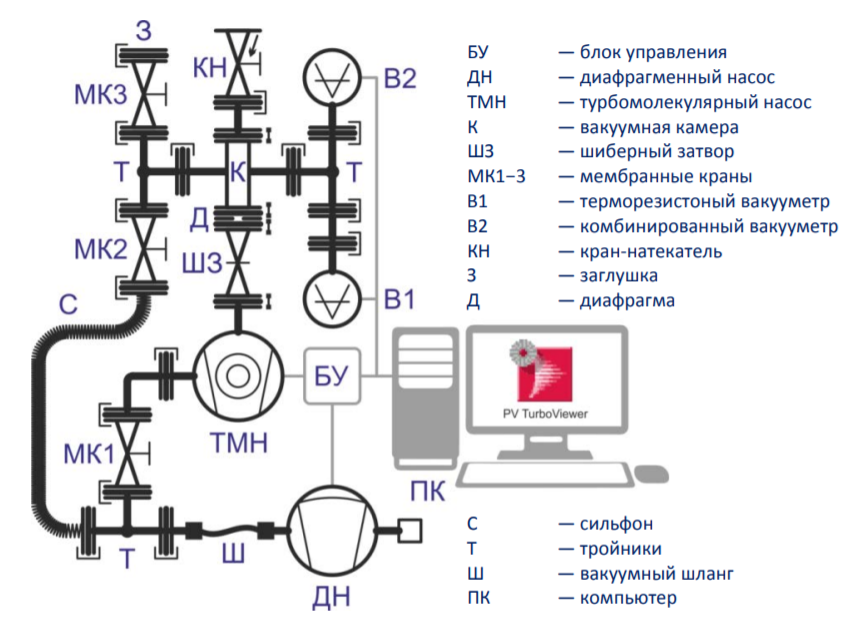
\includegraphics[width=\textwidth]{Схема2.png}
\end{center}
\caption{Схема экспериментальной установки} \label{схема2}
\end{figure}


\begin{figure}[h!]
\begin{center}
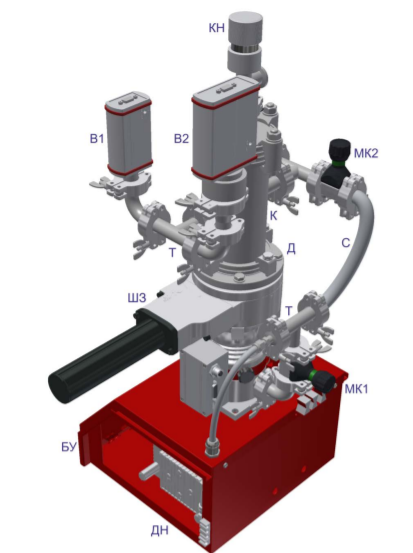
\includegraphics[width=\textwidth]{Схема}
\end{center}
\caption{Модель экспериментальной установки} \label{схема}
\end{figure}

\section{Обработка данных и измерения}
\subsection{Измерение объемов установки}
Откачаем установку до вакуума, подсоединим к ней сильфон (объемом 265 мл), измерим установившееся давление, проделаем эти же действия еще раз и получим значения для объемов частей установки исходя из постоянства температуры (табл. \ref{объемы})

\begin{table}
\caption{Объемы частей системы}
\label{объемы}
\begin{tabular}{|c|c|c|c|}
\hline 
Часть & Объем, мл & $\sigma_V$, мл &$ \epsilon_V$, \% \\ 
\hline 
Камера & 1060 & 50 & 5 \\ 
\hline 
Турмолекулярный насос& 570 & 15 & 3\\ 
\hline 
Вакуумная магистраль & 70 & 5 & 7\\ 
\hline  
\end{tabular} 
\end{table}
\subsection{Измерение пропускной способности форвакуумного насоса}
Рассмотрим две откачки установки форвакуумным насосом. Построим график зависимости давления от времени (рис. \ref{форвакуумный}, табл. \ref{откачка+форв})

Характеристики откачки можно получить по основному уравнению вакуумной техники:
\begin{equation}
\frac{1}{S_0} = \frac{1}{S_H}+\frac{1}{U} 
\end{equation}

\begin{figure}[h!]
\begin{center}
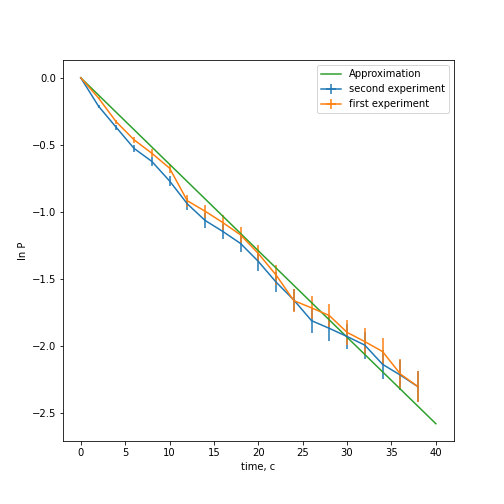
\includegraphics[width=\textwidth]{Форвакуумный}
\end{center}
\caption{Зависимость давления от времени для откачки форвакуумным насосом} \label{форвакуумный}
\end{figure}

\begin{table}
\caption{Характеристики откачки форвакуумным насосом}
\label{откачка+форв}
\begin{tabular}{|c|c|c|c|}
\hline 
$\tau$, c & $S_0$, мл/с& $S_H$, мл/с& U, мл/с  \\ 
\hline 
15.5 $\pm$ 0.8 & 70 $\pm$ 5 & 140 & 130 $\pm$ 10\\ 
\hline  
\end{tabular} 
\end{table}


\subsection{Измерение пропускной способности турбомолекулярного насоса}
Рассмотрим две откачки установки турбомолекулярным насосом. Построим график зависимости давления от времени (рис. \ref{турбомолекулярный}, табл. \ref{откачка+тмн})

Характеристики откачки можно получить по основному уравнению вакуумной техники:
\begin{equation}
\frac{1}{S_0} = \frac{1}{S_H}+\frac{1}{U} 
\end{equation}

\begin{figure}[h!]
\begin{center}
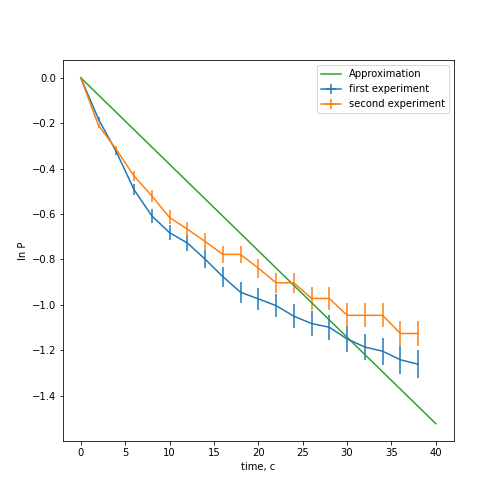
\includegraphics[width=\textwidth]{ТМН}
\end{center}
\caption{Зависимость давления от времени для откачки турбомолекулярным насосом} \label{турбомолекулярный}
\end{figure}

\begin{table}
\caption{Характеристики откачки турбомолекулярным насосом}
\label{откачка+тмн}
\begin{tabular}{|c|c|c|c|}
\hline 
$\tau$, c & $S_0$, мл/с& $S_H$, мл/с& U, мл/с  \\ 
\hline 
26.3 $\pm$ 1.8 & 40 $\pm$ 3 & 60000 & 40 $\pm$ 3\\ 
\hline  
\end{tabular} 
\end{table}


\subsection{Измерения характеристик откачки турбомолекулярным насосом с разными диафрагмами}
Рассмотрим две откачки с диафрагмами с разными диаметрами отверстий (10 мм и 3 мм) (рис. \ref{диафрагма+график} и табл. \ref{диафрагма+табл})

\begin{figure}[h!]
\begin{center}
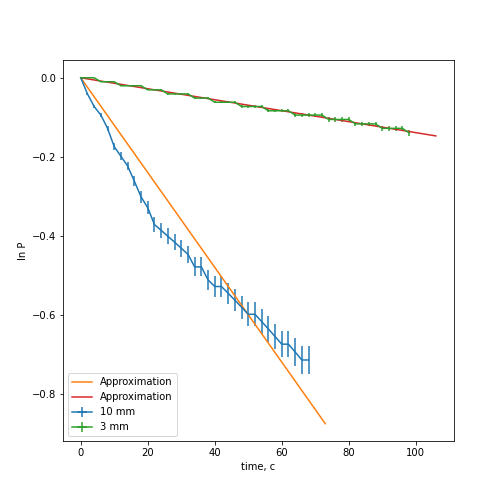
\includegraphics[width=\textwidth]{ТМН+диафрагма.png}
\end{center}
\caption{Зависимость давления от времени для откачки турбомолекулярным насосом с диафрагмой} \label{диафрагма+график}
\end{figure}

\begin{table}
\caption{Характеристики откачки турбомолекулярным насосом через диафрагму}
\label{диафрагма+табл}
\begin{tabular}{|c|c|c|c|c|}
\hline 
Диаметр отверстия, мм&$\tau$, c & $S_0$, мл/с& $S_H$, мл/с& U, мл/с  \\ 
\hline 
10 & 83 $\pm$ 4 & 13 $\pm$ 1 & 60000 & 13 $\pm$ 1\\ 
\hline 
3 & 720 $\pm$ 30 & 1.5 $\pm$ 0.1 & 60000 & 1.5 $\pm$ 0.1\\ 
\hline
\end{tabular} 
\end{table}

Для проводимости отверстия справделиво:
\begin{equation}
U_{\text{отв}} \sim R^2 \sqrt{\frac{T}{m}}
\end{equation}
Проверим, справедлива ли данная формула для полученных данных:
\begin{equation}
\frac{U_1}{U_2}\cdot \frac{R_1^2}{R_2^2} =1.038\approx 1
\end{equation}
Отсюда получается, что формулы справедливы для полученных данных.


\subsection{Оценка уровней течей}

Найдем натекание при закрытии насоса шлюзом, используя значения давления в эти моменты (рис. \ref{течи})
\begin{equation}
Q_H = V\frac{P_K-P_H}{\Delta t} = (31 \pm 3) \cdot 10^{-7} \text{Дж/с}
\end{equation}


\begin{figure}[h!]
\begin{center}
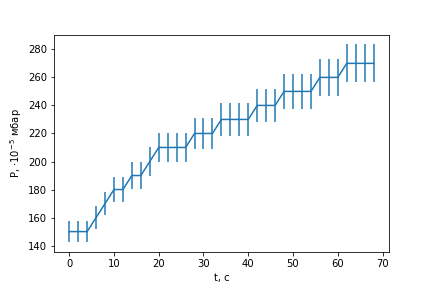
\includegraphics[width=\textwidth]{Течи.png}
\end{center}
\caption{Зависимость давления от времени после перекрытия откачки шибером} \label{течи}
\end{figure}

Проверим допустимость натекания:
\begin{equation}
(31 \pm 3) \cdot 10^{-7} \text{Дж/с} = Q_H \ll Q = P_1 S_0 = 0.006 \text{Дж/с}
\end{equation}

Вследствие этого неравенства натекание в системе можно считать допустимым.

\subsection{Оценка числа Кнудсена для предельных давлений}
Рассчитаем число Кнудсена для предельных давлений по формуле:
\begin{equation}
Kn=\frac{\lambda}{d}=\frac{1}{\sqrt{2}nd\sigma}=\frac{kT}{\sqrt{2}d\sigma p}
\end{equation}
где $\sigma = 1.06 \cdot 10^{-19} м^2$ 
Тогда получим следующие значения для числа Кнудсена (считая диаметр магисрали порядка 1 см): (табл. \ref{кнудсен})


\begin{table}
\caption{Число Кнудсена для предельных давлений}
\label{кнудсен}
\begin{tabular}{|c|c|c|}
\hline 
Часть установки & $P, мбар$ & $Kn$  \\ 
\hline 
Форвакуумная магистарль &  3.6 & $7.5\cdot 10^{-3}$ \\ 
\hline 
Форвакуумная магистраль & $9.1 \cdot 10^{-6}$  & 2900\\ 
\hline
\end{tabular} 
\end{table}

Откуда получаем, что после откачки турбомолекулярным насосом число Кнудсена $Kn\gg 1$, что свидетельствует о молекулярном (кнудсеновском) режиме течения газа.

\section{Вывод}
Получен вакуум с помощью разных насосов и проведены измерения с помощью вакууметров.

1. Для форвакуумного насоса получены значения откачки: $S_0 = 70 \pm 5  \text{мс/с}, U = 130 \pm 10 \text{мл/с} $; для турбомолекулярного насоса - значения откачки:  $S_0 = 40 \pm 3  \text{мс/с}, U = 40 \pm 3 \text{мл/с} $

2. Для откачки турбомолекулярным насосом с разными диафрагмами проверена справедливость соотношения: $Q_H \sim R^2$ 

3. При перекрытии шлюзом проверена допустимость течей: $Q_H \ll Q = P_1 S_0$

4. Проверено, что после откачки турбомолекулярным насосом движение газа переходит в кнудсеновский режим ($Kn=2900 \gg 1$)

\end{document}
